\section{Instruction Fetch Module}

\begin{figure}[h!]
    \centering
    \vspace{1em}
\scalebox{0.85}{
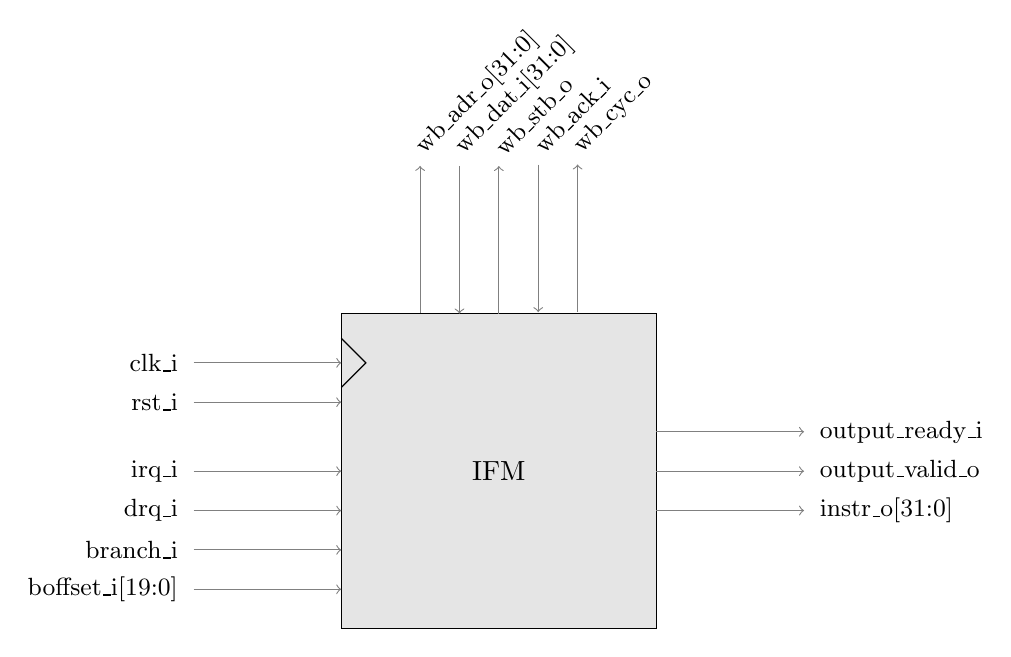
\begin{tikzpicture}[scale=1.25, draw=gray, inner sep=0, outer sep=0]
  \node[rectangle, draw=black,
    anchor=south,
    align=center,
    minimum height = 4cm,
    minimum width = 4cm,
    fill = gray!20] (block) at (0, 0) {IFM};

  \node (rport2) at (block.east) {};
  \node (rport1) at ([yshift=0.4cm]rport2.center) {};
  \node (rport3) at ([yshift=-0.4cm]rport2.center) {};
  \draw[<-] ([xshift=1.5cm]rport1.center) node[right=0.2cm, anchor=west]{\small output\_ready\_i} -- (rport1.center);
  \draw[<-] ([xshift=1.5cm]rport2.center) node[right=0.2cm, anchor=west]{\small output\_valid\_o} -- (rport2.center);
  \draw[<-] ([xshift=1.5cm]rport3.center) node[right=0.2cm, anchor=west]{\small instr\_o[31:0]} -- (rport3.center);

  \node(uport3) at (block.north) {};
  \node(uport2) at ([xshift=-0.4cm]uport3.center) {};
  \node(uport1) at ([xshift=-0.4cm]uport2.center) {};
  \node(uport4) at ([xshift=0.4cm]uport3.north) {};
  \node(uport5) at ([xshift=0.4cm]uport4.center) {};
  \draw[<-] ([yshift=1.5cm]uport1.center) node[above=0.2cm, anchor=west, rotate=45]{\small wb\_adr\_o[31:0]} -- (uport1.center);
  \draw[->] ([yshift=1.5cm]uport2.center) node[above=0.2cm, anchor=west, rotate=45]{\small wb\_dat\_i[31:0]} -- (uport2.center);
  \draw[<-] ([yshift=1.5cm]uport3.center) node[above=0.2cm, anchor=west, rotate=45]{\small wb\_stb\_o} -- (uport3.center);
  \draw[->] ([yshift=1.5cm]uport4.center) node[above=0.2cm, anchor=west, rotate=45]{\small wb\_ack\_i} -- (uport4.center);
  \draw[<-] ([yshift=1.5cm]uport5.center) node[above=0.2cm, anchor=west, rotate=45]{\small wb\_cyc\_o} -- (uport5.center);

  \node (lport2) at ([yshift=-0.4cm]block.west) {};
  \node (lport1) at ([yshift=0.4cm]lport2.center) {};
  \node (lport3) at ([yshift=-0.4cm]lport2.center) {};
  \node (lport4) at ([yshift=-0.4cm]lport3.center) {};

  \draw[->] ([xshift=-1.5cm]lport1.center) node[left=0.2cm, anchor=east]{\small irq\_i} -- (lport1.center);
  \draw[->] ([xshift=-1.5cm]lport2.center) node[left=0.2cm, anchor=east]{\small drq\_i} -- (lport2.center);
  \draw[->] ([xshift=-1.5cm]lport3.center) node[left=0.2cm, anchor=east]{\small branch\_i} -- (lport3.center);
  \draw[->] ([xshift=-1.5cm]lport4.center) node[left=0.2cm, anchor=east]{\small boffset\_i[19:0]} -- (lport4.center);

  \node (clk) at ([yshift=-0.5cm]block.north west) {};
  \draw[->] ([xshift=-1.5cm]lport3.center |- clk.center) node[left=0.2cm, anchor=east]{\small clk\_i} -- (clk.center);
  % clk triangle
  \draw[-  , draw=black] ([yshift=0.25cm]clk.center) -- ([xshift=0.25cm]clk.center) -- ([yshift=-0.25cm]clk.center);

  \node (rst) at ([yshift=-0.4cm]clk.center) {};
  \draw[->] ([xshift=-1.5cm]rst.center) node[left=0.2cm, anchor=east]{\small rst\_i} -- (rst.center);
\end{tikzpicture}
}

    \caption{Schematic view of the Instruction Fetch Module}
    \label{fig:ifm}
\end{figure}

\subsection{Interface}

\begin{content}
The instruction fetch module handles fetching from memory the instructions to be executing. The signals are described in table \ref{tab:ifm-interface}. 
\end{content}

{
  \vspace{0.5em}
  \begin{center}
    \refstepcounter{table}
    Table \thetable: Instruction Fetch Module interface signals\label{tab:ifm-interface}
  \end{center}

\footnotesize
\begin{xltabular}{0.9\textwidth}{|l|c|c|X|}
  \hline
  \cellcolor{gray!20}\textbf{NAME} & \cellcolor{gray!20}\textbf{TYPE} & \cellcolor{gray!20}\textbf{WIDTH} & \cellcolor{gray!20}\textbf{DESCRIPTION} \\
  \hline
  clk\_i & I & 1 & Clock input. \\
  \hline
  rst\_i & I & 1 & Reset input. \\
  \hline
  \multicolumn{4}{|l|}{\textbf{JUMP LOGIC}} \\
  \hline
  irq\_i & I & 1 & External interrupt request. \\
  \hline
  drq\_i & I & 1 & External debug request. \\
  \hline
  branch\_i & I & 1 & Branch request. \\
  \hline
  boffset\_i & I & 20 & Branch offset from the pc of the instruction in the execute stage (pc - 8).  \\
  \hline
  \multicolumn{4}{|l|}{\textbf{WISHBONE MASTER}} \\
  \hline
  wb\_adr\_o & O & 32 & Wishbone read address.  \\
  \hline
  wb\_dat\_i & I & 32 & Wishbone read data. \\
  \hline
  wb\_sel\_o & O & 4 & Wishbone byte selector. \\
  \hline
  wb\_stb\_o & O & 1 & Wishbone handshaking signal asserted when emitting a request. \\
  \hline
  wb\_ack\_i & I & 1 & Acknowledge. Indicates a normal termination of a bus cycle. \\
  \hline
  \multicolumn{4}{|l|}{\textbf{OUTPUT LOGIC}} \\
  \hline
  output\_ready\_i & I & 1 & Output handshaking signal asserted when the destination is ready to receive the output \\
  \hline
  output\_valid\_o & O & 1 & Output handshaking signal asserted when the output is valid. \\
  \hline
  instr\_o & O & 32 & Instruction output. \\
  \hline
\end{xltabular}
}


\subsection{Specification}

\subsubsection{Upstream requirements}

The table \ref{tab:ifm-upstream-requirements} outlines the upstream requirements applicable to the Instruction Fetch Module.

{
  \vspace{0.5em}
  \begin{center}
    \refstepcounter{table}
    Table \thetable: Upstream requirements applicable to the Instruction Fetch Module\label{tab:ifm-upstream-requirements}
  \end{center}
  
\footnotesize
\begin{xltabular}{0.9\textwidth}{|X|c|}
  \hline
  \cellcolor{gray!20}\textbf{ID} \\
  \hline
  \reqref{F\_MEMORY\_INTERFACE\_01} \\
  \hline
\end{xltabular}
}


\subsubsection{Functional requirements}

\paragraph{PC register}

\req{D\_IFM\_PC\_REGISTER\_01}{
  The instruction fetch module shall implement a \texttt{pc} register which shall store the address of the instruction to be fetched.
}[
  derivedfrom=F\_REGISTERS\_03
]

\req{D\_IFM\_PC\_INCREMENT\_01}{
  The value of the \texttt{pc} register shall be incremented by 4 on the rising edge of \texttt{clk\_i} after both \texttt{output\_ready\_i} and \texttt{output\_valid\_o} where asserted.
}

\req{D\_IFM\_PC\_INCREMENT\_02}{
  The value of the \texttt{pc} register shall be incremented by the value of the \texttt{boffset\_i} on the rising edge of \texttt{clk\_i} when \texttt{branch\_i} is asserted.
}


\req{D\_IFM\_PC\_LOAD\_01}{
  The value of the \texttt{pc} register shall be loaded with TBC on the rising edge of \texttt{clk\_i} when \texttt{irq\_i} is asserted.
}

\req{D\_IFM\_PC\_LOAD\_02}{
  The value of the \texttt{pc} register shall be loaded with TBC on the rising edge of \texttt{clk\_i} when \texttt{drq\_i} is asserted.
}

\req{D\_IFM\_PC\_REGISTER\_02}{
  Any changes to the \texttt{pc} register shall be performed before any memory requests.
}

\paragraph{Reset}

\req{D\_IFM\_RESET\_01}{
  The value of the \texttt{pc} register shall be loaded with TBC on the rising edge of \texttt{clk\_i} following the assertion of \texttt{rst\_i}.
}

\req{D\_IFM\_RESET\_02}{
  The \texttt{output\_valid\_o} signal shall be deasserted on the rising edge of \texttt{clk\_i} following the assertion of \texttt{rst\_i}.
}

\paragraph{Fetch triggering}

\req{D\_IFM\_FETCH\_TRIGGER\_01}{
  The instruction fetch module shall perform a memory request on the rising edge of \texttt{clk\_i} following the deassertion of \texttt{rst\_i}.
}

\req{D\_IFM\_FETCH\_TRIGGER\_02}{
  The instruction fetch module shall perform a memory request on the rising edge of \texttt{clk\_i} after both \texttt{output\_ready\_i} and \texttt{output\_valid\_o} are asserted.
}

\paragraph{Memory request}

\req{D\_IFM\_REQUEST\_CANCEL\_01}{
  Any pending memory requests shall be canceled on the rising edge of \texttt{clk\_i} following the assertion of \texttt{rst\_i}.
}

\req{D\_IFM\_REQUEST\_CANCEL\_02}{
  Any pending memory requests shall be canceled on the rising edge of \texttt{clk\_i} following the assertion of \texttt{irq\_i}.
}

\req{D\_IFM\_REQUEST\_CANCEL\_03}{
  Any pending memory requests shall be canceled on the rising edge of \texttt{clk\_i} following the assertion of \texttt{drq\_i}.
}

\req{D\_IFM\_REQUEST\_CANCEL\_04}{
  Any pending memory requests shall be canceled on the rising edge of \texttt{clk\_i} following the assertion of \texttt{branch\_i}.
}

\begin{content}
    The following requirements are extracted from the Wishbone specification for implementing the memory interface of the instruction fetch module.
\end{content}

\req{D\_IFM\_WISHBONE\_DATASHEET\_01}{
  The memory interface shall comply with the Wishbone Datasheet provided in section TBC.
}


\req{D\_IFM\_WISHBONE\_RESET\_01}{
  The memory interface shall initialize itself at the rising edge of \texttt{clk\_i} following the assertion of \texttt{rst\_i}.
}


\req{D\_IFM\_WISHBONE\_RESET\_02}{
  The memory interface shall stay in the initialization state until the rising edge of \texttt{clk\_i} following the deassertion of \texttt{rst\_i}.
}


\req{D\_IFM\_WISHBONE\_RESET\_03}{
  Signals \texttt{wb\_stb\_o} and \texttt{wb\_cyc\_o} shall be deasserted while the memory interface is in the initialization state. The state of all other memory interface signals are undefined in response to a reset cycle.
}[
]

\req{D\_IFM\_WISHBONE\_TRANSFER\_CYCLE\_01}{
  The memory interface shall assert \texttt{wb\_cyc\_o} for the entire duration of the memory access.
}[
  rationale=TBC what wb\_cyc\_o does.
]

\req{D\_IFM\_WISHBONE\_TRANSFER\_CYCLE\_02}{
  Signal \texttt{wb\_cyc\_o} shall be asserted no later than the rising edge of \texttt{clk\_i} that qualifies the assertion of \texttt{wb\_stb\_o}.
}[
]

\req{D\_IFM\_WISHBONE\_TRANSFER\_CYCLE\_03}{
  Signal \texttt{wb\_cyc\_o} shall be deasserted no earlier than the rising edge of \texttt{clk\_i} that qualifies the deassertion of \texttt{wb\_stb\_o}.
}[
]

\req{D\_IFM\_WISHBONE\_ACK\_01}{
  The memory interface shall operate normally when \texttt{ack\_i} is held in the asserted state.
}[
]

\req{D\_IFM\_WISHBONE\_STB\_01}{
  The following signals shall be valid when \texttt{stb\_o} is asserted : \texttt{adr\_o}, \texttt{sel\_o}.
}[
]

\req{D\_IFM\_WISHBONE\_CYCLES\_01}{
  The memory interface shall implement the single read cycle as described in figure \ref{fig:ifm-wishbone-single-read-cycle}.
}[
]

\vspace{0.5em}

\begin{figure}[h!]
    \centering
    \makeatletter\gdef\dividers{}
\begin{tikztimingtable}[%
    scale=0.7,
    timing/dslope=0.1,
    timing/.style={x=6ex,y=3ex},
    x=6ex,
    timing/rowdist=4ex,
    timing/name/.style={font=\footnotesize},
    timing/u/background/.style={fill=gray!20},
    timing/e/background/.style={fill=gray!20},
]
clk\_i & H 3{C C} L \\
adr\_o & 2U 2D{VALID} 4U \\
dat\_i & 2U 2U 2D{VALID} 2U \\
dat\_o & 8U \\
we\_o  & 8L \\
sel\_o & 2U 2D{VALID} 4U \\
stb\_o & 2L 2H 4L \\
ack\_i & 4L 2H 2L \\
cyc\_o & 2L 4H 2L \\
stall\_i & 8L \\
\extracode
% grid
\begin{pgfonlayer}{background}
\begin{scope}[semitransparent ,semithick]
\vertlines[darkgray,dotted]{2, 4, 6}
\dividers
\end{scope}
\end{pgfonlayer}
\end{tikztimingtable}

    \caption{Timing diagram of the single read cycle of the wishbone memory interface}
    \label{fig:ifm-wishbone-single-read-cycle}
\end{figure}

\makeatletter\gdef\dividers{}
\begin{tikztimingtable}[%
    scale=0.7,
    timing/dslope=0.1,
    timing/.style={x=6ex,y=3ex},
    x=6ex,
    timing/rowdist=4ex,
    timing/name/.style={font=\footnotesize},
    timing/u/background/.style={fill=gray!20},
    timing/e/background/.style={fill=gray!20},
]
clk\_i & H 3{C C} L \\
adr\_o & 2U 2D{VALID} 4U \\
dat\_i & 2U 2U 2D{VALID} 2U \\
dat\_o & 8U \\
we\_o  & 8L \\
sel\_o & 2U 2D{VALID} 4U \\
stb\_o & 2L 2H 4L \\
ack\_i & 4L 2H 2L \\
cyc\_o & 2L 4H 2L \\
stall\_i & 8L \\
\extracode
% grid
\begin{pgfonlayer}{background}
\begin{scope}[semitransparent ,semithick]
\vertlines[darkgray,dotted]{2, 4, 6}
\dividers
\end{scope}
\end{pgfonlayer}
\end{tikztimingtable}


\req{D\_IFM\_WISHBONE\_TIMING\_01}{
  The clock input \texttt{clk\_i} shall coordinate all activites for the internal logic within the memory interface. All output signals of the memory interface shall be registered at the rising edge of \texttt{clk\_i}. All input signals of the memory interface shall be stable before the rising edge of \texttt{clk\_i}.
}[
  rationale={As long as the memory interface is designed within the clock domain of \texttt{clk\_i}, the requirement will be satisfied by using the place and route tool.}
]

\paragraph{Output}

\req{D\_IFM\_OUTPUT\_01}{
  The signal \texttt{instr\_o} shall be set to the result of the memory request on the rising edge of \texttt{clk\_i} when the memory request is completed.
}

\req{D\_IFM\_OUTPUT\_02}{
  The signal \texttt{pc\_o} shall be set asynchronously to the value of the \texttt{pc} register.
}

\req{D\_IFM\_OUTPUT\_HANDSHAKE\_01}{
  The signal \texttt{output\_valid\_o} shall be deasserted on the rising edge of \texttt{clk\_i} when the instruction fetch module performs an instruction fetch.
}[
  rationale=Refer to section \ref{control-hazard}.
]

\req{D\_IFM\_OUTPUT\_HANDSHAKE\_02}{
  The signal \texttt{output\_valid\_o} shall be asserted on the rising edge of \texttt{clk\_i} when the instruction fetch is completed.
}[
  rationale=Refer to section \ref{control-hazard}.
]

\req{D\_IFM\_OUTPUT\_HANDSHAKE\_03}{
  When \texttt{output\_valid\_o} is asserted, the instruction fetch module shall hold the value of the \texttt{instr\_o} signal until the rising edge of \texttt{clk\_i} following the assertion of \texttt{output\_ready\_i}.
}[
  rationale=Refer to section \ref{pipeline-stall}.
]

\req{D\_IFM\_OUTPUT\_HANDSHAKE\_04}{
  When \texttt{output\_valid\_o} is asserted, the instruction fetch module shall hold the value of the \texttt{pc\_o} signal until the rising edge of \texttt{clk\_i} following the assertion of \texttt{output\_ready\_i}.
}[
  rationale=Refer to section \ref{pipeline-stall}.
]


\subsection{Behavior}

\begin{content}
  This module doesn't contain any prefetch mechanism as there is no performance requirement for version 1.0.0. This will lead to a performance bottleneck due to the number of cycles needed for fetching instructions from memory.
\end{content}

\subsubsection{Normal behavior}

\begin{content}
  During normal operation, the instruction fetch module sequentially emits memory requests to address stored in the \texttt{pc} register. Upon successful request, \texttt{pc} is incremented to point to the following instruction.

  This behavior induces a pipeline stall due to the delay of the wishbone interface.
\end{content}

\begin{figure}[H]
    \centering
    \makeatletter\gdef\dividers{}
\begin{tikztimingtable}[%
    scale=0.7,
    timing/dslope=0.1,
    timing/.style={x=5ex,y=3ex},
    x=5ex,
    timing/rowdist=4ex,
    timing/name/.style={font=\footnotesize},
    timing/u/background/.style={fill=gray!20},
    timing/e/background/.style={fill=gray!20},
]
clk\_i & H 5{C C} L \\
rst\_i & 2E 8L 2E\\
& \divider{Memory access} \\
wb\_clk\_i & H 5{C C} L \\
  wb\_adr\_o[31:0] & 2.5U 4D{pc} 4D{pc + 4} 1.5U \\
  wb\_dat\_i[31:0] & 4U 2D{mem[pc]} 2U 2D{mem[pc + 4]} 2U \\
wb\_stb\_o & 2.5E 8H 1.5E \\
wb\_ack\_i & 2E 2L 2H 2L 2H 2E \\
& \divider{Stage outputs} \\
output\_ready\_i & 2E 8H 2E \\
output\_valid\_o & 2.5E 2L 2H 2L 2H 1.5E\\
instr\_o[31:0] & 4.5U 2D{mem[pc]} 2U 2D{mem[pc + 4]} 1.5U \\
& \divider{Internal pc value} \\
pc & 2U 4D{pc} 4D{pc + 4} 2U \\
\extracode
% grid
\begin{pgfonlayer}{background}
\begin{scope}[semitransparent ,semithick]
\vertlines[darkgray,dotted]{2, 4, 6, 8, 10}
\dividers
\end{scope}
\end{pgfonlayer}
\end{tikztimingtable}

    \caption{Timing diagram of the normal behavior of the instruction fetch module}
    \label{fig:ifm-behavior-normal}
\end{figure}

\subsubsection{Reset behavior}

\begin{content}
  Once a reset occurs, \texttt{pc} is loaded with the boot address before returning to normal operation.

  This behavior doesn't induce any pipeline stall \textit{per se} as the pipeline is reset during this operation.
\end{content}

\begin{figure}[H]
    \centering
    \begin{tikztimingtable}[%
    scale=0.7,
    timing/dslope=0.1,
    timing/.style={x=5ex,y=3ex},
    x=5ex,
    timing/rowdist=5ex,
    timing/name/.style={font=\footnotesize},
    timing/u/background/.style={fill=gray!20},
    timing/e/background/.style={fill=gray!20},
]
clk\_i & H 7{C C} L \\
rst\_i & 2E 6L 2H 4L 2E\\
wb\_clk\_i & H 7{C C} L \\
  wb\_adr\_o[31:0] & 2U 4D{pc} 2D{pc + 4} 2U 4D{boot\_addr} 2U \\
  wb\_dat\_i[31:0] & 4U 2D{mem[pc]} 2U 2U 2U 2D{a} 2U \\
wb\_stb\_o & 2E 6H 2L 4H 2E \\
wb\_ack\_i & 2E 2L 2H 2L 2L 2L 2H 2E \\
ready\_i & 2E 12H 2E \\
valid\_o & 2E 2L 2H 2L 2L 2L 2H 2E\\
  instr\_o[31:0] & 4U 2D{mem[pc]} 2U 2U 2U 2D{a} 2U \\
\extracode
% grid
\begin{pgfonlayer}{background}
\begin{scope}[semitransparent ,semithick]
\vertlines[darkgray,dotted]{2, 4, 6, 8, 10, 12, 14}
\end{scope}
\end{pgfonlayer}
\end{tikztimingtable}
\begin{center}
  \scriptsize \textit{a : mem[boot\_addr]}
\end{center}

    \caption{Timing diagram of the reset behavior of the instruction fetch module}
    \label{fig:ifm-behavior-reset}
\end{figure}

\subsubsection{Resource busy behavior}

\begin{content}
  The instruction fetch module is capable of handling wait states from memory through the stalling mechanism.
\end{content}

\begin{figure}[H]
    \centering
    \begin{tikztimingtable}[%
    scale=0.7,
    timing/dslope=0.1,
    timing/.style={x=5ex,y=3ex},
    x=5ex,
    timing/rowdist=5ex,
    timing/name/.style={font=\footnotesize},
    timing/u/background/.style={fill=gray!20},
    timing/e/background/.style={fill=gray!20},
]
clk\_i & H 7{C C} L \\
rst\_i & 2E 12L 2E\\
wb\_clk\_i & H 7{C C} L \\
wb\_adr\_o[31:0] & 2U 4D{pc} 8D{pc + 4} 2U \\
wb\_dat\_i[31:0] & 4U 2D{mem[pc]} 2U 2U 2U 2D{mem[pc + 4]} 2U \\
wb\_stb\_o & 2E 12H 2E \\
wb\_ack\_i & 2E 2L 2H 2L 2L 2L 2H 2E \\
ready\_i & 2E 12H 2E \\
valid\_o & 2E 2L 2H 2L 2L 2L 2H 2E\\
  instr\_o[31:0] & 4U 2D{mem[pc]} 2U 2U 2U 2D{mem[pc + 4]} 2U \\
\extracode
% grid
\begin{pgfonlayer}{background}
\begin{scope}[semitransparent ,semithick]
\vertlines[darkgray,dotted]{2, 4, 6, 8, 10, 12, 14}
\end{scope}
\end{pgfonlayer}
\end{tikztimingtable}

    \caption{Timing diagram of the memory resource busy behavior of the instruction fetch module}
    \label{fig:ifm-behavior-wait}
\end{figure}

\subsubsection{Jump behavior}

\begin{content}
  TBC
\end{content}

\begin{figure}[H]
    \centering
    \makeatletter\gdef\dividers{}
\begin{tikztimingtable}[%
    scale=0.7,
    timing/dslope=0.1,
    timing/.style={x=5ex,y=3ex},
    x=5ex,
    timing/rowdist=4ex,
    timing/name/.style={font=\footnotesize},
    timing/u/background/.style={fill=gray!20},
    timing/e/background/.style={fill=gray!20},
]
clk\_i & H 7{C C} L \\
rst\_i & 2E 12L 2E\\
& \divider{Jump inputs} \\
branch\_i & \\
boffset\_i[19:0] & \\
& \divider{Memory access} \\
wb\_clk\_i & H 7{C C} L \\
  wb\_adr\_o[31:0] & 2.5U 4D{pc} 4D{pc + 4} 4D{pc + 8} 1.5U \\
  wb\_dat\_i[31:0] & 4U 2D{mem[pc]} 2U 2D{mem[pc + 4]} 2U 2D{mem[pc + 8]} 2U \\
wb\_stb\_o & 2.5E 12H 1.5E \\
wb\_ack\_i & 2E 2L 2H 2L 2H 2L 2H 2E \\
& \divider{Stage outputs} \\
output\_ready\_i & 2E 12H 2E \\
output\_valid\_o & 2.5E 2L 2H 2L 2H 2L 2H 1.5E\\
instr\_o[31:0] & 4.5U 2D{mem[pc]} 2U 2D{mem[pc + 4]} 2U 2D{mem[pc + 8]} 1.5U \\
\extracode
% grid
\begin{pgfonlayer}{background}
\begin{scope}[semitransparent ,semithick]
\vertlines[darkgray,dotted]{2, 4, 6, 8, 10, 12, 14}
\dividers
\end{scope}
\end{pgfonlayer}
\end{tikztimingtable}

    \caption{Timing diagram of the jump behavior of the instruction fetch module for branch events}
    \label{fig:ifm-behavior-branch}
\end{figure}

\begin{figure}[H]
    \centering
    \input{arch/figures/ifm-behavior-jump-interrupt.tex}
    \caption{Timing diagram of the jump behavior of the instruction fetch module for interrupt events}
    \label{fig:ifm-behavior-interrupt}
\end{figure}

\subsubsection{Hazard behaviors}

\begin{content}
  Hazard behaviors are described in section \ref{pipeline-stall}.
\end{content}

\newpage
